
Freefly-hypyllä putoamisnopeus on keskimäärin 240 km/h, nopeus vaihtelee lentoasennosta riippuen. Tämän vuoksi varusteiden on oltava erinomaisessa kunnossa. Pää- tai varavarjon tahaton aukeaminen kesken freefly-hyppyä voi johtaa vakavaan vaaratilanteeseen. Suuri nopeus aiheuttaa myös sen, että pienetkin vartalon liikkeet aiheuttavat suuria liikkumisia vapaassa. Yhteentörmäysriski on siis suurempi, mikäli et hallitse vartalosi liikkeestä johtuvaa liikkumista vapaapudotuksessa. Törmäämiset vapaassa suurella nopeudella saattavat vahingoittaa sinua tai toista hyppääjää vakavasti. Tässä luvussa käsitellään muun muassa edellä mainittuja turvallisuuteen liittyviä asioita. 

\section{ Varusteet }
\label{turvallisuus-freehyppaamisessa-varusteet}

\subsection{ Reppu-valjasyhdistelmä }
\label{turvallisuus-freehyppaamisessa-reppu-valjasyhdistelma}


Huolehdi, että laskuvarjosi on hyvässä kunnossa. Laskuvarjokokonaisuuden suositellaan täyttävän seuraavat vaatimukset freefly-hypylle: 

\begin{itemize}
\item  Sen tulee sopia hyvin ja tiukasti hyppääjän päälle. Valjaat eivät saa olla niin löysästi puettuna, että ne valuvat hartioilta alas tai jalkahihnat karkaavat kohti polvia. Pahimmassa tapauksessa tällöin on riskinä putoaminen valjaista avauksessa. 
\item  Rintahihnan tulee olla tiukemmalla kuin normaalisti, eikä sen lukitus saa luistaa. Mikäli pää- tai varavarjo aukeaa tahattomasti freefly-hypyn aikana, saattavat tiukemmalla olleet hihnat estää sinua putoamasta valjaista.  
\item  Repun olkaläpät suojaavat kantohihnoja ilmavirralta. Niiden tulee olla tarpeeksi jäykät ja työnnettävissä syvälle lukitukseensa. Ilmavirta saattaa repiä esimerkiksi ohjauslenkin irti kantohihnan kiinnikkeestä, mikäli kantohihnat ovat alttiina ilmavirralle huonosti kiinni pysyvän olkaläpän vuoksi. Velcro-tarroilla suljettavat olkatarrat eivät sovellu freefly-hypyille. 
\item  Pää- ja varavarjon läppien tulee olla jäykät ja ne eivät saa aueta ilmavirran voimasta. 
\item  Irtipäästöpampulan ja varavarjon kahvan velcro-tarrojen tulee olla hyvässä kunnossa, jotta ne pysyvät vapaan aikana kiinnityksissään, eivätkä irtoa freefly-hypyn liikkeitä tehdessäsi. 
\item  Pää- ja varavarjon looppien tulee olla kireät ja ehyet, jotta reppu pysyy suljettuna liikkuessasi eri asennoissa taivaalla. 
\item  Jalkahihnojen välillä suositellaan käytettäväksi elastista kuminauhaa, jotta jalkahihnat eivät liikkuisi vapaan aikana. Varsinkin sittishypyllä jalkahihnat saattavat luisua pois paikoiltaan ja valua polvia kohti. 
\item  Apuvarjon yhdyspunoksen tulisi olla kokonaan piilossa ilmavirralta päävarjon läppien alla, jotta ilmavirta ei pääse repimään apuvarjoa ulos taskustaan. 
\item  Apuvarjon taskun tulee olla kireä ja ehyt sekä apuvarjon tulee olla pakattu taskuunsa siten, että ilmavirta ei revi apuvarjoa ulos taskusta. 
\end{itemize}

Freefly-hypyllä ei suositella käytettäväksi reppu-valjas-yhdistelmää: 

\begin{itemize}
\item  jossa on kaksoispinni joko pää- tai varavarjossa, freefly-liikkeet saattavat avata pinnin tai pinnit 
\item  jossa apuvarjo on joko reisi- tai vatsahihnassa, freefly-liikkeet saattavat irrottaa apuvarjon ulos taskustaan ilmavirralle alttiiksi  
\item  jolla pää- ja varavarjon läpät tai kantohihnojen suojaläpät suljetaan velcro-tarralla. 
\item  jonka apuvarjon yhdyspunos on näkyvillä ja alttiina ilmavirralle, luupin ja apuvarjon taskun välillä. Ilmavirta saattaa repiä yhdyspunoksesta repun auki ja aiheuttaa \textit{hevosenkenkä}-vaaratilanteen. 
\end{itemize}

Oppilaskalustoa saa käyttää vain kouluttajan luvalla. 

\subsection{ Muut varusteet }
\label{turvallisuus-freehyppaamisessa-muut-varusteet}


Freefly-hypyllä muiden varusteiden osalta on huomioitava seuraavia asioita, jotka ovat joko pakollisia tai suositeltavia: 

\begin{itemize}
\item  Suojalasien (goggles) tulee olla ehyet ja niiden kiinnityskuminauhan kireä. Ilmavirta tulee freefly-hypyllä eri suunnasta kuin olet tottunut ja saattaa aiheuttaa suojalasien lähtemisen kesken hypyn 
\item  Kova kypärä yhteentörmäyksien varalta 
\item  Pakollisena visuaalisena mittarina suositellaan käytettäväksi käsimittaria, opettele katsomaan korkeutta mittarista eri lentoasennoissa vapaapudotuksen aikana. 
\item  Äänikorkeusmittarin käyttö on suositeltavaa. Jopa kahta äänikorkeusmittaria voi käyttää. Älä luota pelkästään äänikorkeusmittariisi. 
\item  Kuvaajille suositellaan kuvauskypärään yhden kahvan irtipäästöjärjestelmää 
\item  Varavarjon automaattilaukaisin on erittäin suositeltava ja ennen D-lisenssiä pakollinen 
\item  Vältä vaatteita, jotka saattavat peittää päävarjon avausjärjestelmän, päävarjon irtipäästöpampulan tai varavarjon kahvan vapaassa. 
\item  Koukkupuukon on oltava helposti saatavilla (kuten muissakin hyppylajeissa). 
\end{itemize}
\section{ Toiminta uloshypyssä }
\label{turvallisuus-freehyppaamisessa-toiminta-uloshypyssa}


Suositeltava minimi uloshyppykorkeus freefly-hypyllä on yli 3000 m. Uloshyppykorkeuden ollessa yli 3000 m ehditään suorittaa liikkeitä vapaassa sekä samalla säilyttäen mahdollisuus turvalliseen purkukorkeuteen. Uloshyppyjärjestyksessä suositetaan, että ensin koneesta poistuvat vatsa alaspäin hyppäävät, jonka jälkeen freefly-hyppääjät. Freefly-hyppääjistä liukujat lähtevät viimeisenä. Vatsallaan hyppäävät lähtevät ensimmäisenä, koska he ajautuvat periaatteessa pisimpään vapaan aikana lentolinjaan nähden. Hyppyjärjestys saattaa vaihdella kerhokohtaisesti, joten muista tarkistaa hyppyjärjestys vieraillessasi uudella kerholla. Ylätuulien ollessa kovat hyppäävien ryhmien väliin tulee jättää riittävät välit, ettei vapaan aikana ajauduta edellä tai jälkeen hypänneen ryhmän sekaan vapaassa. Riittävän välin jättämisellä pyritään välttämään päällekkäisiä avauksia eri hyppäävien ryhmien kesken. 


Freefly-hypyillä suunnitellaan useasti erilaisia uloshyppyjä, joissa hyppääjä ottaa otteen toisen hyppääjän raajasta, vaatetuksesta tai valjaista. Suunnittele ja harjoittele uloshyppy jo maassa samalla ottaen huomioon, ettei uloshypyssä otettava ote tai raajan liike pääse repimään vahingossa esimerkiksi varavarjon kahvaa irti kiinnityksestään tai hyppykaverisi apuvarjoa ulos taskusta. 


\begin{figure*}[]\centering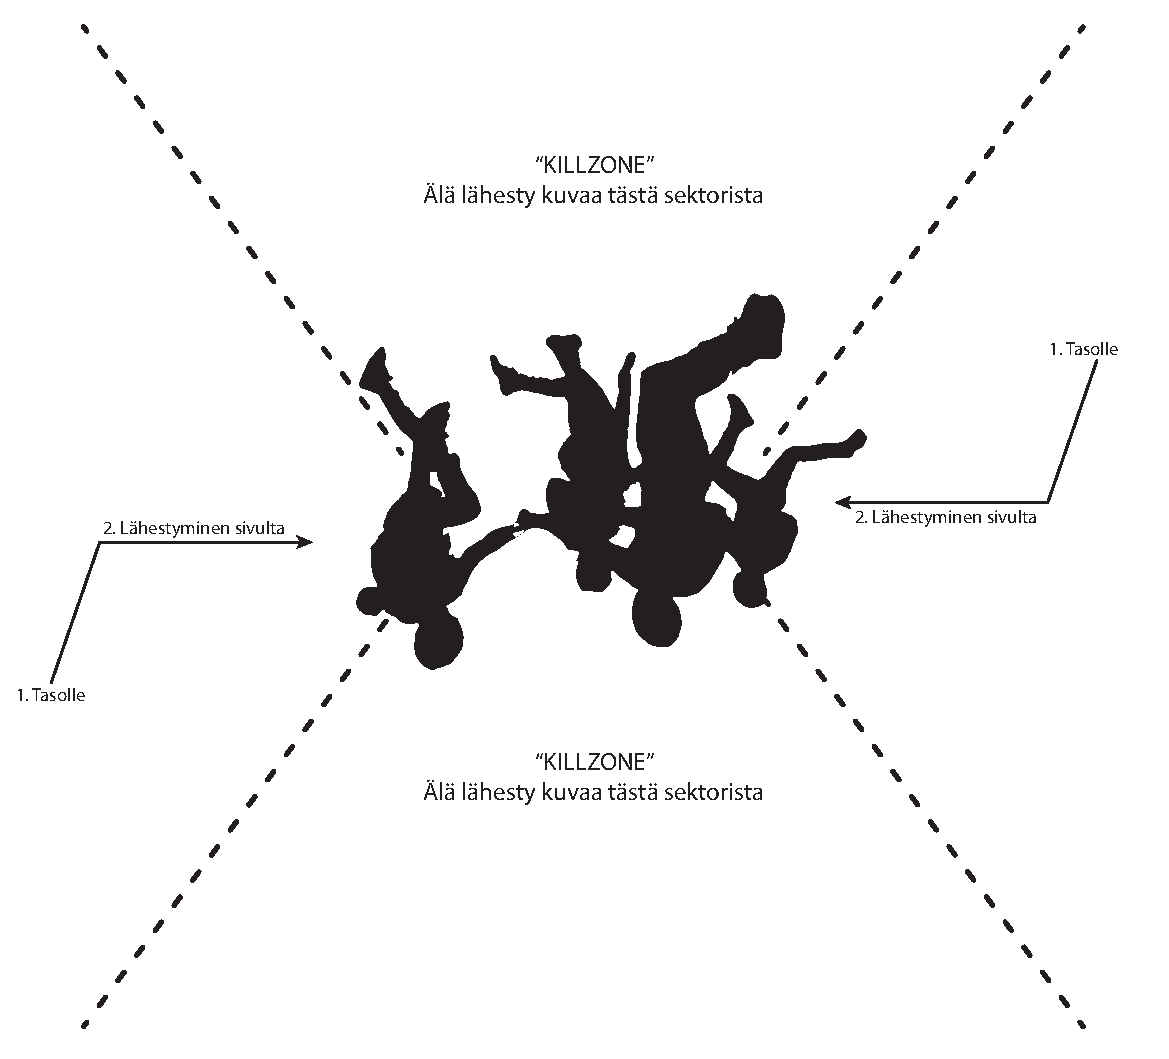
\includegraphics[width=0.8\textwidth]{Killzone.pdf}\caption{Lähesty muodostelmaa aina turvallisesta suunnasta.}\end{figure*} 

\section{ Toiminta vapaassa }
\label{turvallisuus-freehyppaamisessa-toiminta-vapaassa}


Freefly-hypyllä on huomioitava, että putoamisvauhti on huomattavasti kovempi kuin vatsallaan pudotessa. Tämän vuoksi vaakasuuntainen liike hyppylinjaan nähden on freefly-hypyllä suurempi, mikäli hyppääjät eivät putoa suoraan alaspäin. Kuten millä tahansa hypyllä, korkeuden tarkkailu on tärkeää. Huomioi, että 4000 metristä vapaapudotuksen kesto 1000 metrin avauskorkeuteen on noin 45–55 sekuntia, kun vatsallaan lentäen se on noin 60–70 sekuntia. 


Pyri suorittamaan freefly-harjoitukset hyppylinjaan nähden poikittain, hyppäsit sitten yksin tai ryhmässä. Näin vältät tahattoman ajautumisen vapaassa edeltävien tai jälkeesi hypänneiden hyppääjien sekaan. 


Kun hyppäät ryhmässä, pyri säilyttämään visuaalinen kontakti kaikkiin ryhmän hyppääjiin. Opettele lentämään paikallaan sittis- ja hetukka-asennoissa. Lentotason eroja tulee välttää freefly-hypyllä, eli pyri putoamaan samalla horisontaalisella tasolla kuin muut ryhmän hyppääjät. Freefly-ryhmähypylle on hyvä sopia pohja, jonka mukaan muut ryhmän hyppääjät sovittavat putoamisvauhtinsa. Sovitun pohjan puuttuminen saattaa aiheuttaa useita eri tasoja, jotka purkukorkeudessa aiheuttavat vaaratilanteita, koska hyppääjät eivät välttämättä näe, missä kukin on. Sovi aina pohja, jonka mukaan lennetään ryhmähypyllä. 


Älä hyppää isommissa ryhmissä kuin pystyt havainnoimaan, lähde vain taitotasoasi vastaaviin hyppyihin! Ei ole häpeä jäädä pois erityistä taitoa vaativilta hypyiltä sen sijaan, että osallistut ja taitamattomuuttasi pilaat muiden hypyn tai pahimmassa tapauksessa vahingoitat kanssahyppääjää. 


Mikäli ajaudut freefly-hypyllä ryhmän ylä- tai alapuolelle, ota vaakatasossa eroa muihin ryhmän hyppääjiin säilyttäen katsekontaktin ryhmään ja hankkiudu ryhmän sivulla samalla tasolle. Lähesty ryhmää vain samalta tasolta sivusta. Älä koskaan lähesty putoavaa freefly-hyppääjien muodostelmaa suoraan päältä tai alta! Lähestyessäsi sivulta vältät suurinopeuksisen törmäyksen vaaran, mikäli joku alla olevista esimerkiksi korkkaa. Opettele siis palloasento suurinopeuksisia törmäyksiä välttääksesi. 


Vältä freefly-ryhmähypyllä pilveen hyppäämistä. Mikäli kuitenkin joudut pilveen vapaan aikana, pyri säilyttämään katsekontakti muihin ryhmän hyppääjiin. Jos menetät katsekontaktin, pyri putoamaan paikallaan. Älä käännä putoamisasentoa vatsalleen, koska joku voi olla yläpuolellasi. Pilvestä pois päästyäsi tarkista ilmatila ja korkeudesta riippuen pura hyppy turvalliseen suuntaan tai lennä muun ryhmän luokse. 


Hypättäessä liukuhyppyä soolona tai ryhmähyppynä, on liukumissuunta ja oletettu varjojen avaamisalue suunniteltava siten, että ne sijoittuvat selvästi erilleen aikaisemmin hypänneiden hyppääjien hyppylinjasta. Älä koskaan suuntaa liukua suoraan hyppylinjan päälle tai aikaisemmin hypänneiden hyppääjien yläpuolelle! 

\section{ Törmääminen vapaassa }
\label{turvallisuus-freehyppaamisessa-tormaaminen-vapaassa}


Vältä kovavauhtista törmäämistä kaikin mahdollisin keinoin. Voit välttää törmäyksen menemällä palloasentoon ajoissa, jolloin kovavauhtinen liike eteen- tai taaksepäin yleensä pysähtyy. Varaudu kuitenkin törmäykseen, mikäli et tee palloasentoa ajoissa. Yritä kaikin keinoin välttää törmäämistä vapaassa erityisesti pää edellä. Mikäli törmäät vapaassa, suojele päätäsi ja ota törmäys vastaan raajoillasi (mikäli mahdollista). Tarkista törmäyksen jälkeen itsesi, varusteesi ja kaverisi. Mikäli loukkasit itsesi tai varusteissasi ilmenee poikkeavaa, pura hyppy ja keskity avaamiseen. 

\section{ Toiminta purkukorkeudessa ja varjon avaamisen jälkeen }
\label{turvallisuus-freehyppaamisessa-toiminta-purkukorkeudessa-ja-varjon-avaamisen-jalkeen}


Purkumerkki ja -korkeus on sovittava maassa ennen freefly-ryhmähyppyä. Tällöin jokainen hyppääjä voi asettaa äänikorkeusmittarin asetuksen purkukorkeudelle. Purkukorkeus kannattaa määrittää ryhmän koon ja kokemuksen mukaan. Epätietoisuus muiden sijainnista purussa freefly-ryhmähypyillä saattaa johtaa päällekkäisiin avauksiin tai törmäämisiin vapaassa. Välttääksesi näitä tilanteita, pura freefly-ryhmähyppy sovitussa korkeudessa. Nyrkkisääntö: mitä enemmän hyppääjiä on mukana ryhmässä, sitä korkeammalla hypyn muodostelma tulee purkaa. Ohessa esimerkkejä suositeltavista purkukorkeuksista: 

\begin{itemize}
\item  2 - 4 hyppääjää, 1400 m 
\item  yli 4 hyppääjää, 1500 m 
\item  yli 8 hyppääjää, 1600 m  
\item  yli 12 hyppääjää, 1700 m tai enemmän 
\end{itemize}

Ennen freefly-ryhmähypyn purkua pyri saamaan näköyhteys kaikkiin mukana olleisiin hyppääjiin. Jos et näe purkumerkin jälkeen kaikkia ryhmässä hypänneitä, tee paikallasi 180 asteen käännös ja pyri löytämään loput hyppääjät. Liu´u tämän jälkeen vapaaseen suuntaan. 


Sittishypyllä on tärkeää saada purkumerkin jälkeen etäisyyttä lähellä oleviin hyppääjiin. Purkumerkin jälkeen peruuta varoen ensin pois kuvasta sittiksessä ja käänny vasta sen jälkeen liukuun. Peruuttaminen on tärkeää, jotta et potkaise hyppykaveriasi kääntyessäsi liukuasentoon. Peruuttaessa riskinä on kuitenkin se, että takanasi onkin toinen hyppääjä. 


Hetukkahypyllä voit liukua pois muodostelmasta kahdella eri tavalla. Ensimmäinen tapa on liukua niin, että pystyasennon kulmaa muuttaa loivasti mahallaan liukumiseen. Tätä tapaa voit käyttää silloin, kun olet varma, ettei selän takana ole ketään. Tee liukumisen aikana tynnyri, jolloin tarkastat yläpuolisen ilmatilan vapaana olon. Tämän jälkeen pysäytä liuku, tarkasta ylä- ja alapuolinen ilmatila avausmerkkiä tehdessäsi ja avaa varjosi. Tynnyrin tekemistä liukumisen aikana kannattaa harjoitella soolohypyillä. On tärkeää ettei liukumisen suunta muutu tynnyriä tehdessä. 


Toinen ja suositeltavampi tapa suorittaa purku ja liuku hetukkahypyllä on tehdä purkumerkin jälkeen hallittu 180 asteen käännös pois ryhmän keskustasta, jonka jälkeen lähdetään loivasti kiihdyttäen poispäin ryhmästä selkäliu´ulla tarkastaen samalla yläpuolinen ilmatila. Selkäliuku käännetään vatsaliukuun siinä vaiheessa kun on saatu riittävästi etäisyyttä muihin hyppääjiin. Pysäytä liuku, tarkasta ylä- ja alapuolinen ilmatila avausmerkkiä tehdessäsi ja avaa varjosi. Erityisesti tässä purkutekniikassa korkeuden tarkkailu on tärkeää, koska hallittu käännös ja selkäliukuun lähteminen vie aikaa. 


Jos huomaat avauskorkeudessa toisen hyppääjän alapuolellasi, tarkasta yläpuolinen ilmatilasi ja avaa varjosi välittömästi. Mikäli alla oleva hyppääjä on jo avaamassa varjoa tai näet allasi avautuvan varjon, pyri liukumaan tehokkaasti ohi tai sivulle välttääksesi törmäyksen. 


Avattuasi varjon tarkasta ilmatila ja käännä varjosi takimmaisista kantohihnoista lentämään poikittain hyppylinjaan nähden. Lähde lentämään kohti alastuloaluetta vasta sen jälkeen, kun olet saanut havainnon edelläsi ja jälkeesi hypänneistä hyppääjistä sekä omasta ryhmästäsi varjon varassa. Tällä toimenpiteellä saatat ehkäistä päällekkäisiä avauksia ja törmäyksiä vapaassa olevien ja varjon varassa olevien hyppääjien välillä. 


\begin{figure*}[]\centering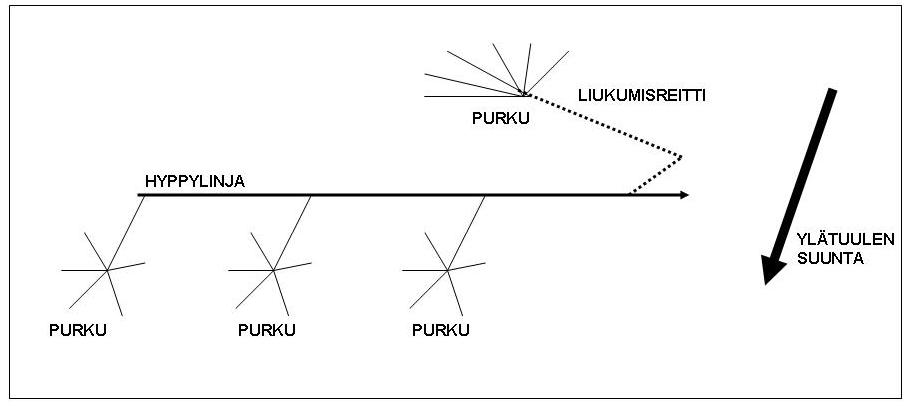
\includegraphics[width=0.8\textwidth]{Liukumislinja-viimeisena-sivutuuli.jpeg}\caption{Liukumaan lähtenyt ryhmä hyppää ulos linjan viimeisenä sivutuulilinjalla.}\end{figure*} \begin{figure*}[]\centering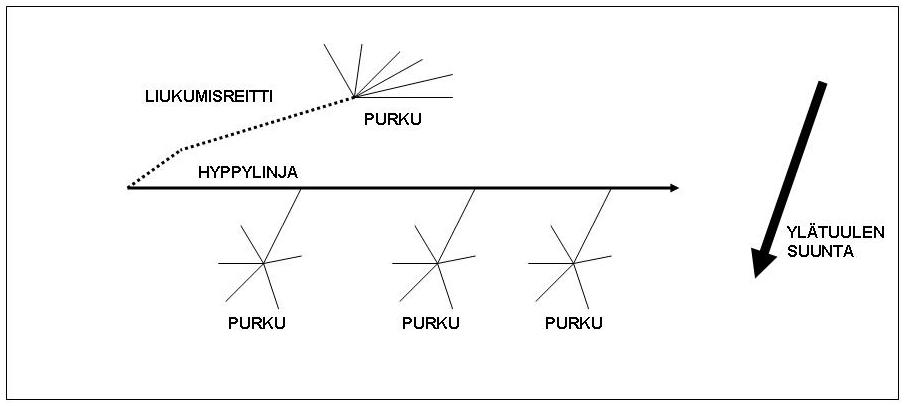
\includegraphics[width=0.8\textwidth]{Liukumislinja-ensimmaisena.jpeg}\caption{Liukumaan lähtenyt ryhmä hyppää ulos linjan ensimmäisenä sivutuulilinjalla.}\end{figure*} \begin{figure*}[]\centering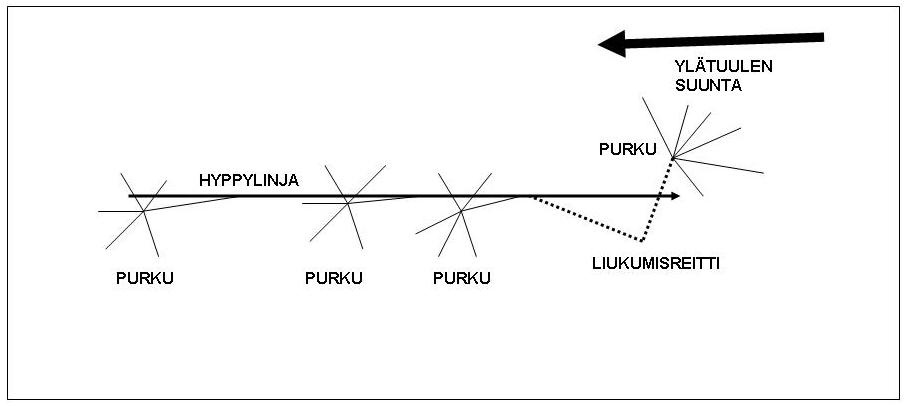
\includegraphics[width=0.8\textwidth]{Liukumislinja-viimeisena-vastatuuli.jpeg}\caption{Liukumaan lähtenyt ryhmä hyppää ulos linjan viimeisenä vastatuulilinjalla.}\end{figure*} 

\section{ Kulmahypyn suunnittelu }
\label{turvallisuus-freehyppaamisessa-kulmahypyn-suunnittelu}


Kun aloitat kulmahypyn suunnittelun, sinulla tulee olla ajantasaiset tuulitiedot. Tee liukusuunnitelma vallitsevien tuulten mukaan jo maassa äläkä suunnittele liukuvasi liian kauas. Jos pilvet estävät suunnistamisen, älä hyppää liukuhyppyä. Perusideana on suunnitella hyppy siten, että avauksessa hyppääjät ovat ylätuulen puolella hyppylinjaan nähden ja riittävän etäällä muista hyppylinjan ryhmistä (ks. alla olevat kuvat). Suuntaa päätettäessä kannattaa huomioida myös mahdolliset varalaskupaikat. Liukuryhmässä tulee aina olla yksi hyppääjä, (leader) joka vastaa liu´un pysymisestä suunnitellulla reitillä. Kulmaryhmän leaderin tulisi olla kokenut kulmailija. Suunta voidaan katsoa maastosta, koneesta tai auringosta. Maastoa käytettäessä on luonnollisesti tarpeen tuntea kentän lähiympäristö, jotta oikea liukusuunta löytyy helposti. Selkäliukuja voi aluksi katsoa suunnan koneesta, mikä on hyvä keino pilvisellä säällä. 


Kulmaryhmät sijoitetaan useimmiten linjan loppuun ja joskus myös linjan alkuun. Muista selvittää, onko samassa pokassa muitakin kulmaryhmiä ja sopikaa yhdessä, mihin suuntaan kukin ryhmä liikkuu. Soololiukujia saatetaan joskus sijoittaa myös keskelle hyppylinjaa, jolloin on tärkeää liikkua aina poikki hyppylinjan. 


Kulmahypyn purkukorkeus sovitaan aina ennen hypylle lähtöä. Mitä enemmän hyppääjiä ryhmässä on ja mitä kauemmaksi liu´utaan tuulenvoimakkuus huomioon ottaen, sitä aikaisemmassa vaiheessa aloitetaan purku. Yleensä kulmahypyt puretaan normaalia korkeammalla (1600–2000 m). Purussa lähdetään liukumaan omalta paikalta sovittuun suuntaan, yleensä viistoittain sivuun. Kuvittele ajavasi moottoritiellä, jolta lähdet liittymässä pois. Yli 90 asteen käännöksen voit tehdä vain, jos olet täysin varma, ettei takanasi ole ketään. Jos jäät kulmahypyn aikana reilusti jälkeen muista, lähde ajoissa pois ja ota välimatkaa muihin liukumatta kuitenkaan takaisin hyppylinjan päälle. Tämä sovitaan jo maassa ennen hypylle lähtöä. 

\section{ Turvallisuuteen liittyvä termejä }
\label{turvallisuus-freehyppaamisessa-turvallisuuteen-liittyva-termeja}

\subsection{ Korkkaus }
\label{turvallisuus-freehyppaamisessa-korkkaus}


Jos pitelet korkkia veden alla ja päästät siitä irti, korkki singahtaa pintaan. Korkkaus (Corking) on ympäri maailman yleinen ilmaisu, jolla kuvataan kovassa vauhdissa olevan hyppääjän lentoasennon kontrolloimatonta ja äkillistä muutosta huomattavasti hitaampaan lentoasentoon (esimerkiksi hetukka-asento vaihtuu äkisti vatsalleen). Normaali vauhti vatsa alaspäin on noin 200km/h kun taas freefly-vauhti on yleensä noin 240km/h, usein paljon enemmänkin. Jos hyppääjä korkkaa yllättäen hypyn aikana, hän voi osua yläpuolellaan oleviin hyppääjiin niin suurella vauhdilla, että siitä voi seurata vakava loukkaantuminen tai jopa kuolema. 

\subsection{ Palloasento }
\label{turvallisuus-freehyppaamisessa-palloasento}


Korkkaamisen mahdollisuuden vuoksi on tärkeää harjoitella säilyttämään vauhti samana, vaikka asento ei pysyisikään haluamanasi. Hyvä keino tähän on palloasento (Recovery Position/Ball Position). Palloasennossa jalat ovat koukussa, reidet rintaa vasten, selkä pyöreänä ja kädet varpaita kohden. Ilmavirran tulee osua tässä asennossa hyppääjän alaselän alueelle. Asentoa voi tasapainottaa myös sivuille levitetyillä käsillä etenkin noustessa palloasennosta sittikseen. Palloasentoa voit harjoitella maassa selällään nostaen jalat ja kädet ylös. Harjoittele tämä myös ilmassa. Ennen kuin aloitat hetukkaharjoittelun, sinun pitää hallita korkanneen asennon palauttaminen joko palloasennon kautta sittikseen tai mieluummin suoraan sittikseen, sillä sittiksessä et sinkoile holtittomasti, vaan pystyt lentämään paikoillaan ja samaa nopeutta kuin muu ryhmä. Lisäksi sittiksessä ympäristön havainnointi on helpompaa kuin palloasennossa. Palloasentoa onkin syytä käyttää opetellessa sittistä. 


\begin{Figure}\centering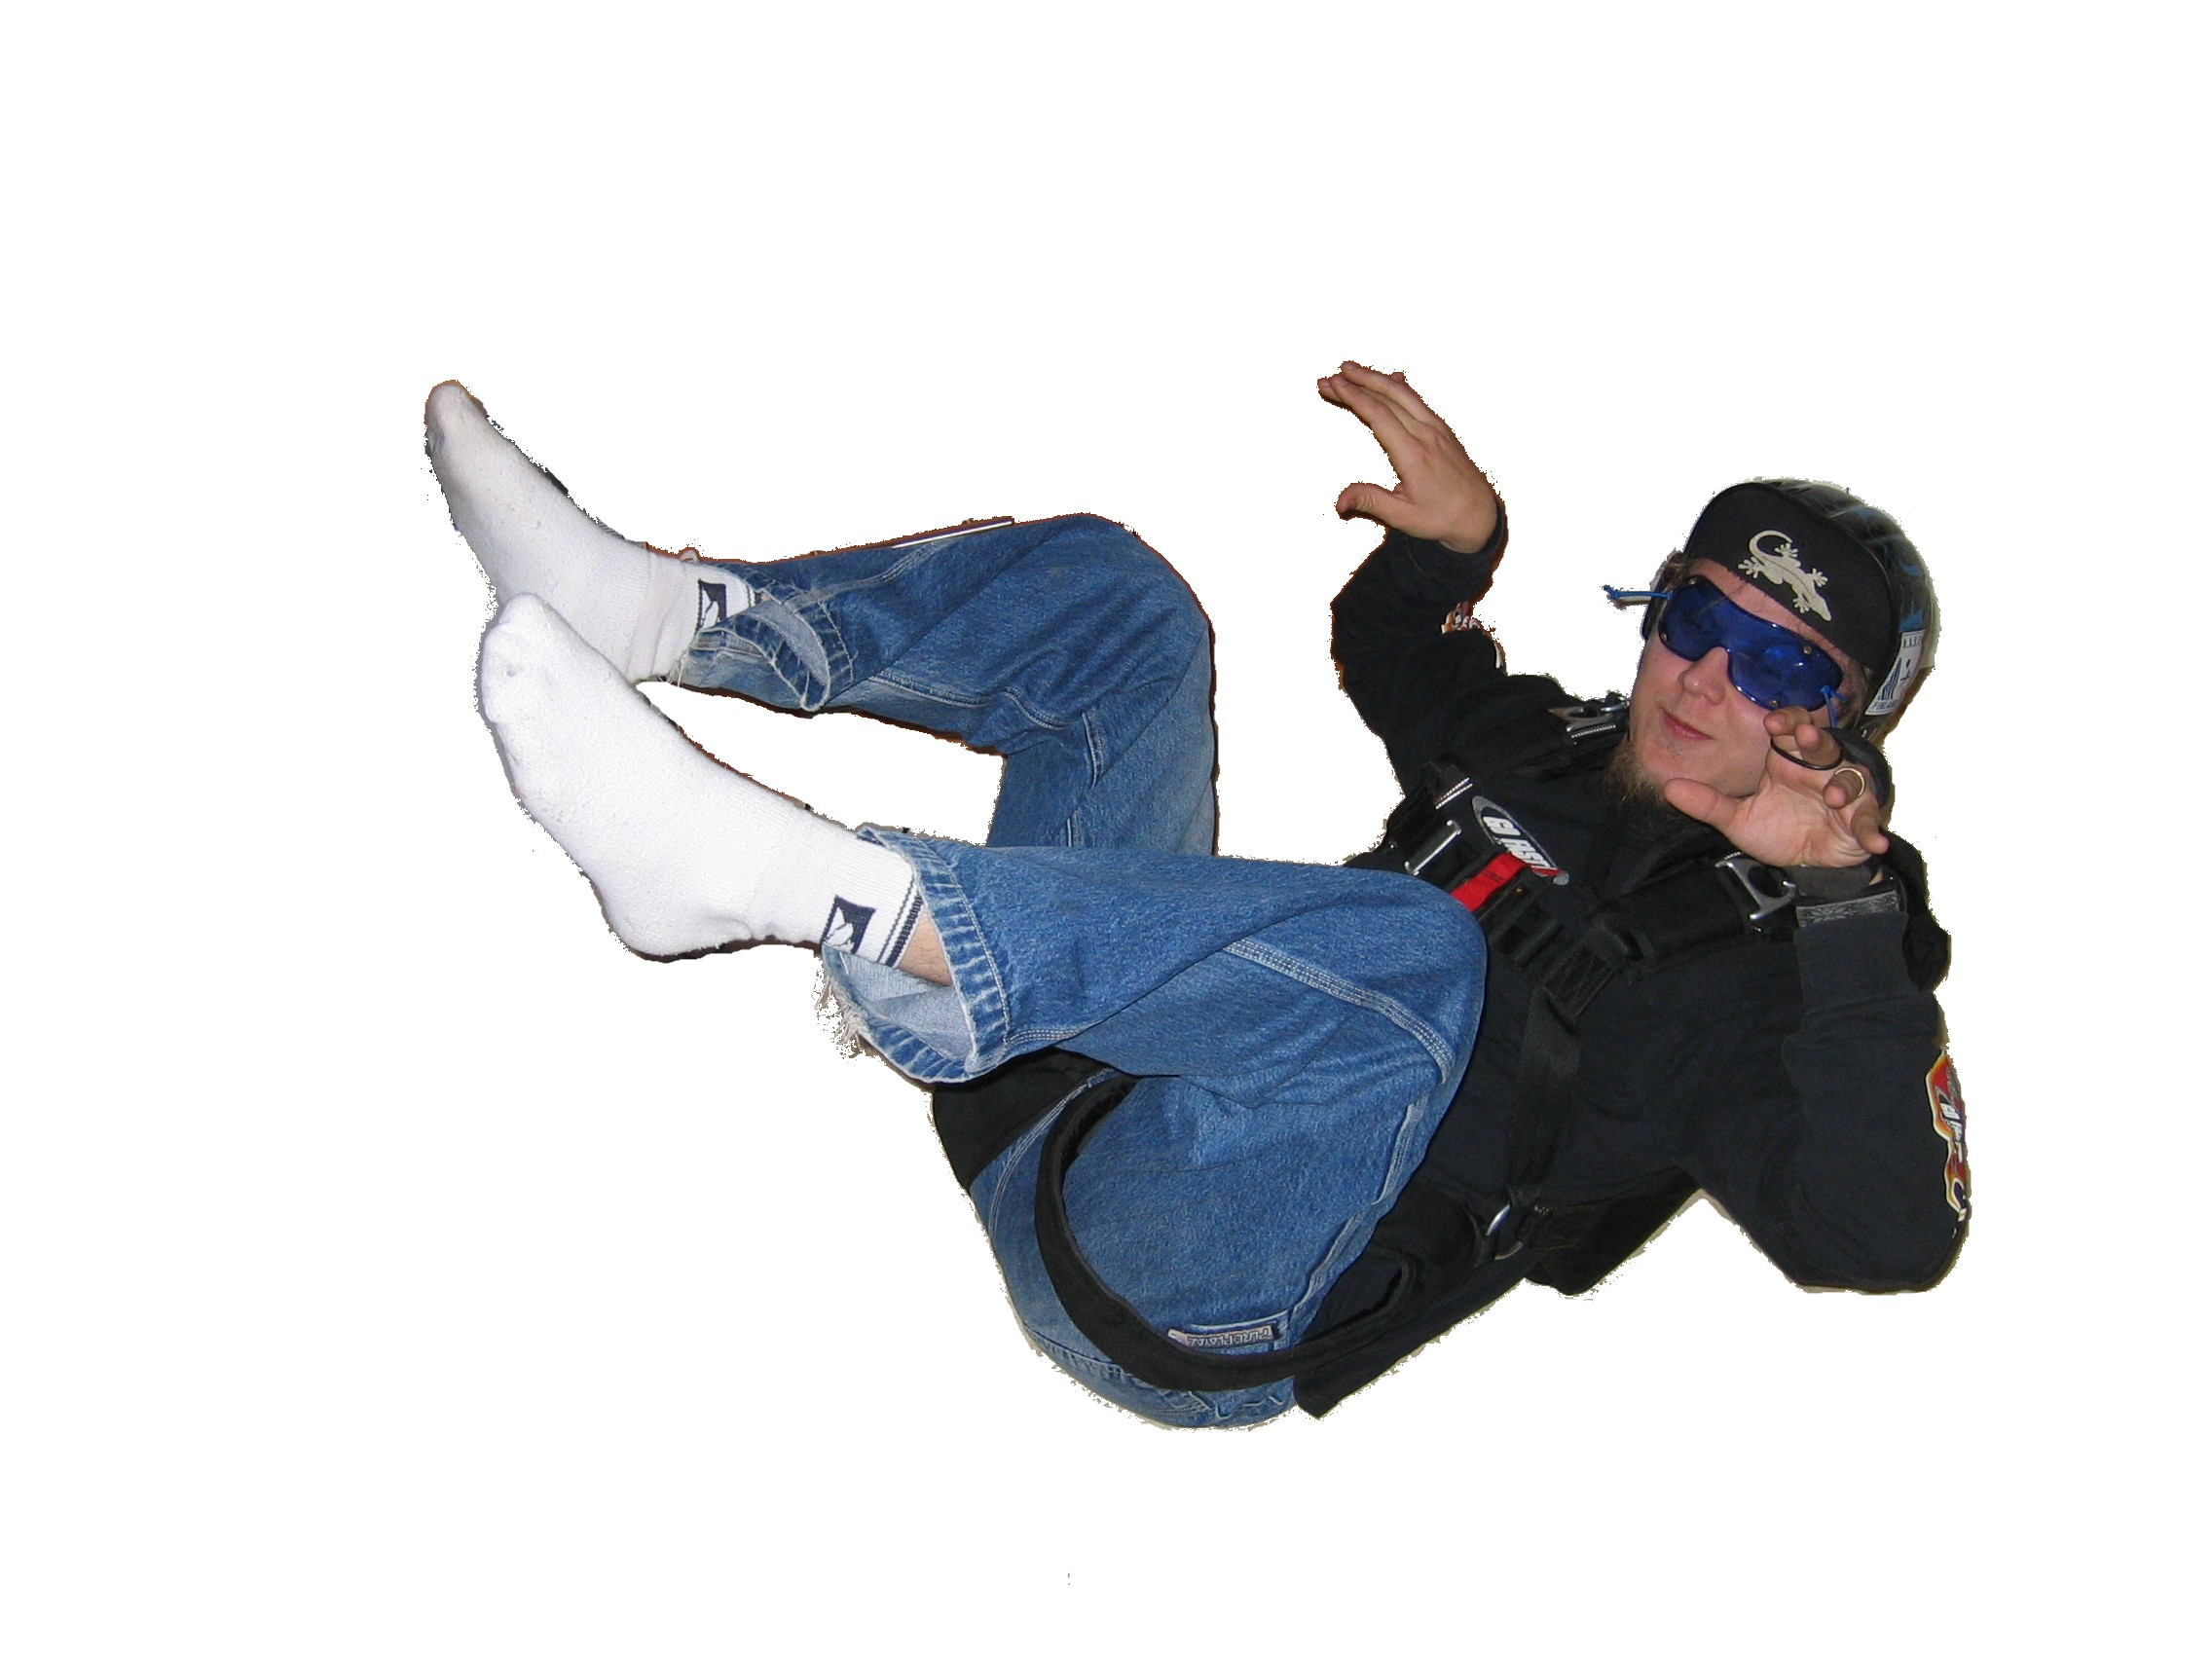
\includegraphics[width=0.9\textwidth]{FFRecoveryPosition.jpg}\captionof{figure}{Freefly Recovery Position}\end{Figure} 

\subsection{ Tahaton liikkuminen vapaassa }
\label{turvallisuus-freehyppaamisessa-tahaton-liikkuminen-vapaassa}


Kun aloitat harjoittelun, liikut tietämättäsi varsin paljon. (Zooming) Erityisesti hetukkahypyllä liikkuminen voi pahimmillaan olla liukumista jyrkässä kulmassa. Tietääksesi liikkuuko hyppyasentosi eteen tai taaksepäin voit pyytää mukaan kokeneempaa hyppääjää, joka osaa lentää paikallaan. Hän näkee, liikutko tahattomasti eteen- tai taaksepäin vai pysytkö paikallasi. Voit tehdä samanlaisen harjoituksen myös hyppykaverin kanssa, mikäli hän pysyy paikallaan sittiksessä. 

\subsection{ Kiertäminen }
\label{turvallisuus-freehyppaamisessa-kiertaminen}


Kiertäminen (Orbiting) syntyy, kun kaksi hyppääjää lentää toisiaan kohti, mutta eivät pysäytä eteenpäin menevää liikettä. Ohittaessaan toisensa he kääntävät katseensa toisiaan kohden, mutta eteenpäin menevä liike jatkuu. Hyppääjien vartalot kääntyvät katseesta johtuen kohti keskustaa ja eteenpäin menevän liikkeen suunta muuttuu vartalon kierron mukana, jolloin hyppääjät alkavat kiertää kuviteltua keskustaa. 


Kiertämisen voit lopettaa pysäyttämällä itsesi ja ottamalla horisontista kiintopisteen. Jos kaverisi liikkuu, älä seuraa häntä, vaan tee esimerkiksi 90 asteen hallittu käännös siinä vaiheessa, kun hyppykaveri katoaa näköpiiristä. Etsi tämän jälkeen uusi kiintopiste ja yritä pysyä paikoillaan. Kiertäminen ei ole suuri turvallisuusriski, mikäli hypätään kahdestaan. Suuremmissa ryhmissä hypättäessä se saattaa aiheuttaa ongelmia. Siirtyessäsi hyppäämään isompia kuvia on tärkeää osata pysyä paikallaan. 

